\documentclass[10pt, a4paper,spanish]{article}
\usepackage[utf8]{inputenc}

\usepackage{varwidth}
\usepackage{graphicx}

\usepackage[T1]{fontenc} % Use 8-bit encoding that has 256 glyphs
\usepackage{microtype} % Slightly tweak font spacing for aesthetics

\usepackage[hmarginratio=1:1,top=32mm,columnsep=20pt]{geometry} % Document margins
\usepackage[hang, small,labelfont=bf,up,textfont=it,up]{caption} % Custom captions under/above floats in tables or figures
\usepackage{float} % Required for tables and figures in the multi-column environment - they need to be placed in specific locations with the [H] (e.g. \begin{table}[H])
\usepackage{hyperref} % For hyperlinks in the PDF

\usepackage{abstract} % Allows abstract customization
\renewcommand{\abstractnamefont}{\normalfont\bfseries} % Set the "Abstract" text to bold
\renewcommand{\abstracttextfont}{\normalfont\small\itshape} % Set the abstract itself to small italic text

\usepackage{titlesec} % Allows customization of titles
\renewcommand\thesection{\Roman{section}} % Roman numerals for the sections
\renewcommand\thesubsection{\Roman{subsection}} % Roman numerals for subsections
\titleformat{\section}[block]{\large\scshape\centering}{\thesection.}{1em}{} % Change the look of the section titles
\titleformat{\subsection}[block]{\large}{\thesubsection.}{1em}{} % Change the look of the section titles

\usepackage{fancyhdr} % Headers and footers
\pagestyle{fancy} % All pages have headers and footers
\fancyhead{} % Blank out the default header
\fancyfoot{} % Blank out the default footer
\fancyhead[C]{ Marzo 2016 $\bullet$ JumpVa $\bullet$ Análisis de la Aplicación} % Custom header text
\fancyfoot[RO,LE]{\thepage} % Custom footer text

%----------------------------------------------------------------------------------------
%	TITLE SECTION
%----------------------------------------------------------------------------------------

\title{\vspace{-15mm}\fontsize{24pt}{10pt}\selectfont\textbf{Mapa del Sitio}} % Article title

\author{
\large
\textsc{Alberto Amigo Alonso\textsubscript{20\%}}\\[2mm] % Your name
\textsc{Sergio Delgado Álvarez\textsubscript{20\%}}\\[2mm] % Your name
\textsc{Sergio García Prado\textsubscript{20\%}}\\[2mm] % Your name
\textsc{Oscar Fernández Angulo\textsubscript{20\%}}\\[2mm] % Your name
\textsc{Silvia Rodriguez Ares\textsubscript{20\%}}\\[2mm] % Your name
\normalsize Universidad de Valladolid \\ % Your institution
\vspace{-5mm}
}
\date{}

%----------------------------------------------------------------------------------------

\begin{document}

	\maketitle % Insert title

	\thispagestyle{fancy} % All pages have headers and footers

%----------------------------------------------------------------------------------------
%	ABSTRACT
%----------------------------------------------------------------------------------------

	\begin{abstract}
		\noindent Servicio web destinado a permitir a remitentes y destinatarios ofertar envíos para que los transportistas sean capaces de encontrarlos permitiendo a todos los usuarios monitorizarlos.
	\end{abstract}

%----------------------------------------------------------------------------------------
%	TEXT
%----------------------------------------------------------------------------------------
	\section{Mapa del sitio:}


		\begin{figure}[H]
			\centering
				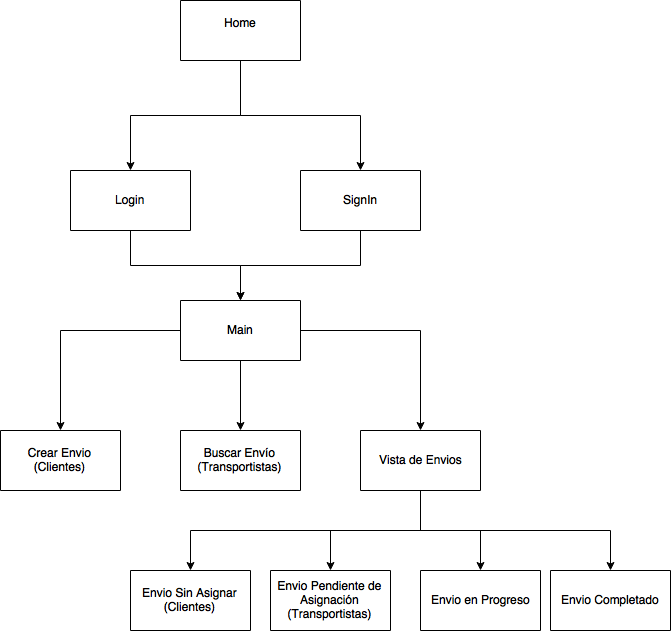
\includegraphics[width=0.75\textwidth]{sitemap.png}
		\end{figure}

	\section{Guía de Uso}

		\paragraph{}
		Dado que la página web está hecha con Angular.js y se ha utilizado una única página raíz en la cual se van incluyendo las distintas partes según convenga, para probar la página hay que ejecutar \textbf{web/index.html}.

		\paragraph{}
		En esta primera vista podemos encontrar dos botones azules, que sirven para crearse una cuenta e iniciar sesión en el sistema. Al no tener que implementar la funcionalidad del sistema (aunque buena parte ha sido adelantada), se han habilitado dos botones verdes de muestra para poder simular los casos de hacer login con una cuenta de transportista y de cliente.

		\paragraph{}
		La página de inicio es muy similar para efectos del transportista y del cliente. En esta vista podemos encontrar los envíos en los que cada uno está participando, con dos diferencias notables:

		\begin{enumerate}
				\item Para los envios sin asignar, los transportistas tienen la etiqueta \textbf{pendiente} mientras que los clientes tienen \textbf{no asignado}.
				\item En la barra superior el cliente tiene la opción de elegir la opción \textbf{crear envío}, desde la que accederá al menú modal con el formulario para solicitar un envío. El transportista, sin embargo, podrá hacer uso de la opción \textbf{buscar envío}, en la que le aparecerán los envíos sobre los que puede pujar.
		\end{enumerate}

		\paragraph{}
		\textit{Importante}: Para probar las distintas funcionalidades del cliente y el transportista, \textbf{cerrar sesión} en vez de usar el botón de atrás del navegador. Esta opción se encuenta pulsando en el nombre del usuario de la esquina superior izquierda. 

\end{document}
